\documentclass{article}
\usepackage[utf8]{inputenc}
\usepackage{fixltx2e}
\usepackage{mathtools}
\usepackage{parskip}
\usepackage{graphicx}
\usepackage{epstopdf}
\usepackage{float}
\usepackage{enumitem}
\usepackage{amsmath}
\usepackage[margin=1in]{geometry}

\makeatletter
\renewcommand*\env@matrix[1][\arraystretch]{%
  \edef\arraystretch{#1}%
  \hskip -\arraycolsep
  \let\@ifnextchar\new@ifnextchar
  \array{*\c@MaxMatrixCols c}}
\makeatother

\title{Zvezda}
\author{Jaime Ernesto Forero Romero \\ Nicolas Rocha Pacheco}
\date{2016}

\begin{document}
\graphicspath{ {images/} }

\maketitle
\tableofcontents
\listoffigures

\section{Introduction}

\begin{figure}[H]
    \centering
    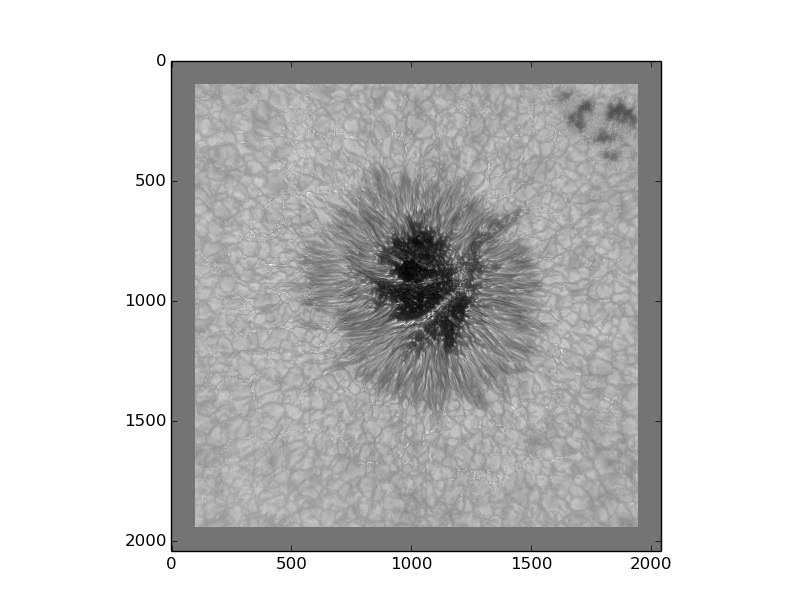
\includegraphics[width=\textwidth]{original}
    \caption{This image was used to test if the algorithm was working}
    \label{image}
\end{figure}

\section{Algorithm}



Since we have been looking for a way to detect the filamentary structures in the sun we had to start with an image of the sun and then do some analysis of that image through the algorithm. The mathematical analysis of the image was done keeping in mind an algorithm developed and previously used by Professor Forero to find filamentary structures on sun’s chromosphere. Since we are working with an image we must use values for each pixel as they were part of an associated function $F(x,y)$ even we can not define them in $x$ or $y$.
The first step was calculating the $2\times2$ Hessian matrix for each pixel as it follows:

\begin{equation}
    H =
    \begin{bmatrix}[2.5]
        \dfrac{\partial^{2} F}{\partial x^{2}} & \dfrac{\partial^{2} F}{\partial x \ \partial y} \\
        \dfrac{\partial^{2} F}{\partial y \ \partial x} & \dfrac{\partial^{2} F}{\partial y^{2}}  
    \end{bmatrix}
\end{equation}

The problem was that as the associated function $F(x,y)$ can not be differentiated with common mathematical rules as it is only defined on integers, we had to use the following numerical approximations of second order derivatives:

\begin{equation}
    \dfrac{\partial^{2} F}{\partial x^{2}} = \dfrac{F(x+h,y) - 2F(x,y) + F(x-h,y)}{h^{2}}
    \label{DerivativeXX}
\end{equation}

\begin{equation}
    \dfrac{\partial^{2} F}{\partial y^{2}} = \dfrac{F(x,y+j) - 2F(x,y) + F(x,y-j)}{j^{2}}
\end{equation}

\begin{equation}
    \frac{\partial^{2} F}{\partial x \partial y} = \dfrac{F(x+h,y+j)-F(x+h,y-j)-F(x-h,y+j)+F(x-h,y-j)}{4hj}
    \label{DerivativeXY}
\end{equation}

Since we are working with differences between pixels $h$ and $j$ are 1 for every numerical approximation except for the pixels from the edge as we can not calculate the derivatives as those pixels do not have surrounding pixels. Once we have the Hessian matrix for each pixel we are encouraged to calculate the eigenvalues of this matrix. During the development of the algorithm we plotted the derivatives as we were able to calculate them.

This is a summary of all the steps in the algorithm:

\begin{enumerate}[label=\textbf{\arabic*}.]
    \item \textbf{Hessian Matrix} The first step was calculate the Hessian matrix for each pixel, so we used finite derivatives as a numerical method to approximate second-order derivatives. As each pixel had it's own Hessian matrix we had to save each Hessian matrix in another matrix that was used later to do some calculations. The Hessian matrix calculation was defined as a function inside the Python script that used the FITS image data as parameter and resulted in a matrix containing the Hessian matrix for each pixel.
    
    \item \textbf{Eigenvalues} Once we had the Hessian matrix for each pixel, we calculated the eigenvalues of each Hessian matrix. With those eigenvalues we created a new matrix where each pixel had it's two associations. Then we made two graphs from that matrix, one containing the first eigenvalue and a second one containing the second eigenvalue. This step was also defined as a function inside Python where the parameter was each Hessian matrix. 
    
    \item \textbf{Histogram} Our final step was plotting the histograms of each eigenvalues, also, we plotted both of them in the same graphic. Finally we took different sections of the image we used to see the difference between different patterns.
    
\end{enumerate}


\section{Results}

\subsection{Full image analysis}

The first test we made was passing the whole image through the algorithm. We started by cutting the edges out of the image as can be seen in Figure \ref{fig:fullAnalyzed}. As we were not interested on analyzing the sunspot, this was just a test on the eigenvalue function.

\begin{figure}[H]
    \centering
    \includegraphics[width=0.5\textwidth]{full/analyzed}
    \caption{Part of the image that was analyzed}
    \label{fig:fullAnalyzed}
\end{figure}

\begin{figure}[H]
    \centering
    \includegraphics[width=0.5\textwidth]{full/first}
    \caption{Resulting image from calculating the first eigenvalues}
    \label{average}
\end{figure}

\begin{figure}[H]
    \centering
    \includegraphics[width=0.5\textwidth]{full/second}
    \caption{Resulting image from calculating the second eigenvalues}
    \label{average}
\end{figure}

\subsection{Lower-left corner}

\begin{figure}[H]
    \centering
    \includegraphics[width=0.5\textwidth]{esqinf/analyzed}
    \caption{Resulting image from calculating the first eigenvalues}
    \label{average}
\end{figure}

\begin{figure}[H]
    \centering
    \includegraphics[width=0.5\textwidth]{esqinf/first}
    \caption{Resulting image from calculating the first eigenvalues}
    \label{average}
\end{figure}

\begin{figure}[H]
    \centering
    \includegraphics[width=0.5\textwidth]{esqinf/second}
    \caption{Resulting image from calculating the second eigenvalues}
    \label{average}
\end{figure}

\section{Future work}



\section{References}

\end{document}
